\begin{figure}
\centering
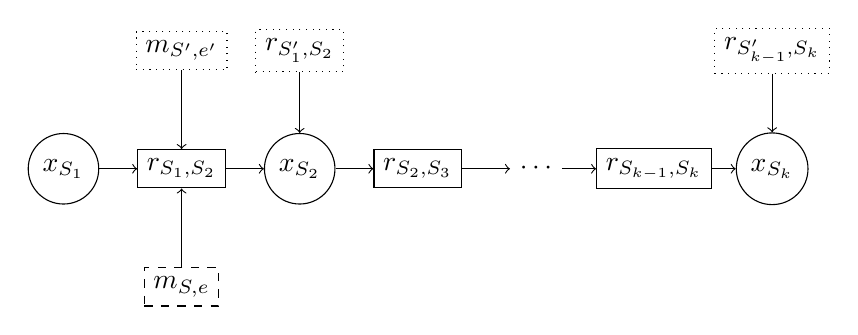
\begin{tikzpicture}
  \tikzset{
    _x/.style={circle,draw},
    r/.style={rectangle,draw},
    m/.style={rectangle,draw,dashed},
    w/.style={rectangle,draw,dotted},
  };
  \node[_x] (x-S1)       at (-1.5,0)  {$x_{S_1}$};
  \node[_x] (x-S2)       at (1.5,0)   {$x_{S_2}$};
  \node[_x] (x-Sk)       at (7.5,0)   {$x_{S_k}$};
  \node[m]  (m-S-e)      at (0,-1.5)  {$m_{S,e}$};
  \node[r]  (r-S1-S2)    at (0,0)     {$r_{S_1,S_2}$};
  \node[r]  (r-S2-S3)    at (3,0)     {$r_{S_2,S_3}$}; 
  \node[r]  (r-Sk-1-Sk)  at (6,0)     {$r_{S_{k-1},S_k}$};
  \node[w]  (m-S'-e')    at (0,1.5)   {$m_{S',e'}$};
  \node[w]  (r-S'1-S2)   at (1.5,1.5) {$r_{S'_1,S_2}$};
  \node[w]  (r-S'k-1-Sk) at (7.5,1.5) {$r_{S'_{k-1},S_k}$};
  \node     (dots)       at (4.5,0)   {$\cdots$};

  \draw[->] (x-S1)       -- (r-S1-S2);
  \draw[->] (m-S-e)      -- (r-S1-S2);
  \draw[->] (m-S'-e')    -- (r-S1-S2);
  \draw[->] (r-S1-S2)    -- (x-S2);
  \draw[->] (r-S'1-S2)   -- (x-S2);
  \draw[->] (x-S2)       -- (r-S2-S3);
  \draw[->] (r-S2-S3)    -- (dots);
  \draw[->] (dots)       -- (r-Sk-1-Sk);
  \draw[->] (r-Sk-1-Sk)  -- (x-Sk);
  \draw[->] (r-S'k-1-Sk) -- (x-Sk);
\end{tikzpicture}
\caption{Elements of $W$}
\label{fig:witness}
\end{figure}
    